\documentclass[oneside,a4paper,10pt]{article}
\usepackage[english,brazilian]{babel}
\usepackage[alf]{abntex2cite}
\usepackage[utf8]{inputenc}
\usepackage[T1]{fontenc}
\usepackage[top=10mm, bottom=10mm, left=10mm, right=10mm]{geometry}
\usepackage{framed}
\usepackage{booktabs}
\usepackage{color}
\usepackage{hyperref}
\usepackage{graphicx}
\usepackage{float}
\usepackage{amssymb} %Símbolos de Conjuntos numéricos
\usepackage{multicol} %Várias Colunas
\graphicspath{{./Figuras/}}    
\definecolor{shadecolor}{rgb}{0.8,0.8,0.8}

\newcommand{\EREM}{EREM Regina Pacis}
\newcommand{\curso}{\textbf{2 EMSI}}
\newcommand{\professor}{Prof. Leandro Vieira}

\newcommand{\PR}[1]{\ensuremath{\left[#1\right]}} %Comandos para parênteses grandes
\newcommand{\PC}[1]{\ensuremath{\left(#1\right)}}
\newcommand{\chav}[1]{\ensuremath{\left\{#1\right\}}}

\begin{document}
\pagestyle{empty}
\textbf{fevereiro de 2020 - at. I: matrizes}

	\begin{center}
		\EREM
		\par %pula uma linha
		\curso
		\par
		\professor
		\par
		\vspace{10pt}
		\textbf{\large{Atividade de Matemática da I Unidade}}
	\end{center}
	
\begin{enumerate}
\item A tabela a seguir mostra os números de desempregados no Brasil de 1999 a 2002 em percentual da população economicamente ativa:

\begin{center}
\begin{tabular}{|c|c|c|c|c|}
\hline 
 & 1999 & 2000 & 2001 & 2002 \\ 
\hline 
Homens & 7,6 & 7,1 & 6,2 & 7,1 \\ 
\hline 
Mulheres & 7,1 & 6,5 & 5,9 & 6,7 \\ 
\hline 
Total & 8,3 & 8,0 & 6,7 & 7,8 \\ 
\hline 
\end{tabular} 
\end{center}

	\begin{enumerate}
	\item Em qual ano o percentual de homens desempregados foi maior?
	\item Em qual ano o percentual de mulheres desempregadas foi o menor?
	\item Em qual ano o percentual total de desempregados foi o maior, e em qual foi o menor?
	\item (Desafio) Sabendo que em 2002 a população brasileira era de 180 milhões, e que a a população economicamente ativa(PEA) nessa época era de 65\% do número de habitantes, calcule o a PEA, e o número de desempregados:
	\end{enumerate}
	
\item A tabela a seguir apresenta dados sobre a receita nas vendas de produtos de uma rede lanchonetes:
\begin{figure}[h]
\center
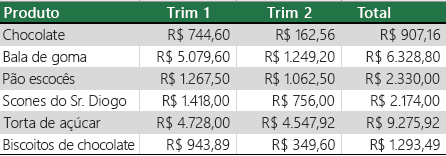
\includegraphics[width=8cm]{Figuras/t1.png}
\label{omeubrowser}
\end{figure}

	\begin{enumerate}
	\item Em qual trimestre a receita foi a maior:
	\item Qual o total da receita para o período observado:
	\item Qual a média das idades dos estudantes dessa turma:
	\item (Desafio) Sabendo que com esses produtos é possível obter um lucro de 20\% sobre a receita, qual o lucro da rede lanchonetes no primeiro e no segundo semestre:
	\item (Desafio) Qual o percentual da receite proveninete da torta de açucar da receita total, para o período observado:
	\end{enumerate}
	
\item A tabela a seguir apresenta as notas dos estudantes de uma turma de engenharia de uma faculdade nas disciplina de estatísticae cálculo:

\begin{figure}[h]
\center
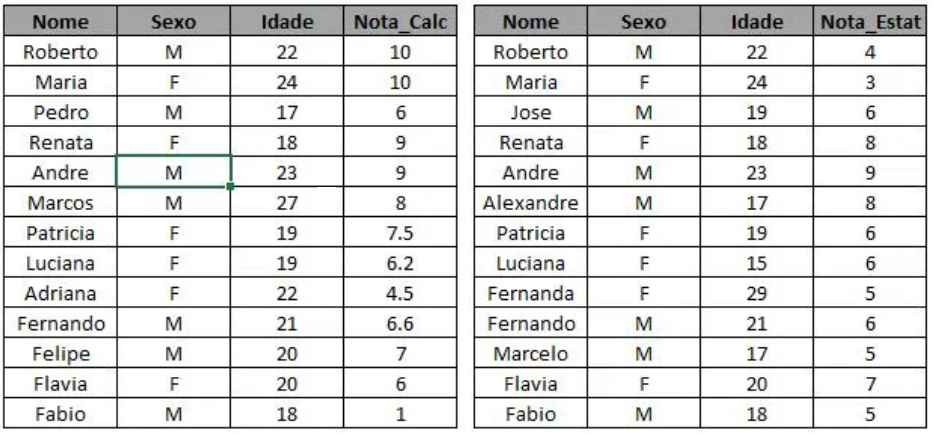
\includegraphics[width=12cm]{Figuras/t2.png}
\label{omeubrowser}
\end{figure}

Com base nas informações contidas na tabela responda aos senguintes ítens:
	\begin{enumerate}
        \item Qual estudante tirou a maior nota em cada uma das disciplinas:
		\item Qual das disciplinas apresenta a maior média da turma:
		\item Sabendo que nessa turma a média de aprovação é 7,0, qual o percentual em cada uma das disciplinas de alunos abaixo da média:
		\item (Desafio) Qual o percentual da turma observada é do sexo feminino? Do total de estudantes mulheres observadas, qual o percentual que está abaixo da média em pelo menos uma disciplina?
	\end{enumerate}	

\item Construa as matrizes reais pedidas:
	\begin{enumerate}
        \item $A_{2\times2} = (a_{ij} = i^2 +j^2)$
		\item $A_{2\times2} = (a_{ij} = i^2 - 2j)$
		\item $A_{3\times3} = (a_{ij} = i+2j)$
	\end{enumerate}		

\item Qual o elemento que se encontra na 1ª linha e na 1ª coluna da Matriz $M_{10 \times 10}=\PC{a_{ij}=i-j}$, e qual o elemento que se encontra na 9ª linha e na 9ª coluna :
	
\item Qual o elemento que se encontra na 5ª linha e na 6ª coluna da Matriz $M_{7 \times 9}=\PC{a_{ij}=3i-j^{2}}$, e qual o elemento que se encontra na 7ª linha e na 8ª coluna :

\item Sejam as matrizes A, B e C a seguir:
\begin{multicols}{3}
$ A = \left[		
\begin{array}{cc}
-1   & 2    \\
2  & 0
\end{array}
\right] $

$ B = \left[		
\begin{array}{cc}
1   & -3    \\
5  & 0
\end{array}
\right] $				

$ C = \left[		
\begin{array}{cc}
0   & 2    \\
-7  & 2
\end{array}
\right] $
\end{multicols}
Calcule:
\begin{multicols}{4}
\begin{enumerate}
\item $A+B$
\item $A-B$
\item $B+C$
\item $C-B$
\end{enumerate}
\end{multicols}

\item Sejam as matrizes A, B e C a seguir:
\begin{multicols}{3}
$ A = \left[		
\begin{array}{cc}
-1   & 2    \\
2  & 0
\end{array}
\right] $

$ B = \left[		
\begin{array}{cc}
1   & -3    \\
5  & 0
\end{array}
\right] $				

$ C = \left[		
\begin{array}{cc}
0   & 2    \\
-7  & 2
\end{array}
\right] $
\end{multicols}
Calcule:
\begin{multicols}{4}
\begin{enumerate}
\item $2A$
\item $2A-3B$
\item $C-4A$
\item $5A-10B$
\end{enumerate}
\end{multicols}
		
\item Dadas as Matrizes $A_{2 \times 2}=\PC{a_{ij}=4i-5j}$ e $B_{2 \times 2}=\PC{a_{ij}=4i-5j}$. Calcule $ 2A - 3B$:
			
\item Dadas as matrizes	A, B e C a seguir calcule o valor de $2A + 3B - 5C$:
\begin{multicols}{3}
		$ A = \left[		
		\begin{array}{ccc}
		-1   & 2    & 0  \\
		2  & 0      & -2 \\
		0   & 3 & 1
		\end{array}
		\right] $
				
		$ B = \left[
		\begin{array}{ccc}
		0   & 1    & -1  \\
		3  & -1      & 2 \\
		0   & 0 & 1
		\end{array}
		\right] $
				
		$ C = \left[		
		\begin{array}{ccc}
		2	& 1    & 0  \\
		0  & -1      & -2 \\
		0   & 1		& 	2
		\end{array}
		\right] $		
\end{multicols}
		
\item Calcule o Determinate das seguintes matrizes:
\begin{multicols}{4}
\begin{enumerate}
 
\item	$ M = \left[		
		\begin{array}{cc}
		-5   & 2  \\
		2  & 0   \\		
		\end{array}
		\right] $
				
\item	$ N = \left[		
		\begin{array}{cc}
		6   & 3  \\
		2  & -6   \\		
		\end{array}
		\right] $
				
\item 	$ O = \left[		
		\begin{array}{cc}
		5   & 4  \\
		1  & -2 \\		
		\end{array}
		\right] $
		
\item	$ P = \left[		
		\begin{array}{cc}
		11   & -15  \\
		21  & 12   \\
		\end{array}
		\right] $
\end{enumerate}		
\end{multicols}
		
\item Use a regra de Cramer (determinantes) para resolver o seguinte sistema 
\begin{multicols}{4}
\begin{enumerate}
\item $\cases{5x+4y=-17 \cr 6x+7y=6}$ 
\item $\cases{11x+12y=22 \cr 31x+22y=-68}$ 
\item $\cases{5x+4y=8 \cr 8x-6y=174}$
\item $\cases{26x+17y=116 \cr 41x+19y=261}$ 
\end{enumerate}
\end{multicols}			
			
\item Calcule o determinante das seguintes matrizes:			
\begin{multicols}{3}
\begin{enumerate}
\item	$ A = \left[		
		\begin{array}{ccc}
		-1   & 2    & 0  \\
		2  & 0      & -2 \\
		0   & 3 & 1
		\end{array}
		\right] $
				
\item	$ B = \left[
		\begin{array}{ccc}
		0   & 1    & -1  \\
		3  & -1      & 2 \\
		0   & 0 & 1
		\end{array}
		\right] $
				
\item	$ C = \left[		
		\begin{array}{ccc}
		2	& 1    & 0  \\
		0  & -1      & -2 \\
		0   & 1		& 	2
		\end{array}
		\right] $
\end{enumerate}	
\end{multicols}			
		
\item Marque no plano o triângulo $ABC$, com $A=(-2,1)$, $B=(-1,3)$ e $C=(3,2)$. Calcule a área do triângulo $ABC$:

\item No plano cartesiano, faça a reta $AB$, onde $A=(-3,1)$ e $B=(2,4)$. E encontre sua equação:

\item Encontre a equação da reta $AB$ que passa nos pontos 	$A=(-5,2)$ e $B=(3,6)$:

\item Encontre a equação da reta $r$, que passa nos pontos $A$ e $B$, onde $A=(3,2)$ e $B=(-1,-5)$:
						
\end{enumerate}

	\vspace{14pt}
	
	\flushbottom
	\flushright
	"Quem nunca errou nunca experimentou nada novo."\\(Albert Einstein)
	
\end{document}
